%chktex-file 36
%chktex-file 23
%chktex-file 10
%chktex-file 17
%chktex-file 9
\documentclass[computationalMathematics.tex]{subfiles}

%%%%%%%%%%%%%%~~~~~~~~~~~~~~~~~~~~~~~~~~~~~~~~~~~~~~~~%%%%%%%%%%%%%%%
\chapter{25th of October 2018}
\chapterauthor{A. Frangioni}
%%%%%%%%%%%%%%~~~~~~~~~~~~~~~~~~~~~~~~~~~~~~~~~~~~~~~~%%%%%%%%%%%%%%%

\recap{During last lecture we started dealing with algorithms for performing a line search for the minimum of $\varphi$, in particular we introduced first order algorithms.}

\subsubsection{Second order algorithms}

\begin{theorem}
  Given $f : \R^n \to \R$ such that $f \in \C{2}$ and let $\varphi(\alpha) = \vect{x} + \alpha \vect{d}$,  $\exists \varphi''(\alpha) = \tr{\vect{d}} \nabla^{2} f(\vect{x} + \alpha \vect{d} ) \vect{d}$ and it is continuous.
\end{theorem}

\begin{proof}
	\[
	\begin{split}
		\parder{\ps{\nabla f(\vect{x} + \alpha \vect{d})}{\vect{d}}}{\alpha} &= \parder{\ps{\vect{d}}{\nabla f(\vect{x} + \alpha \vect{d})}}{\alpha}\\
		&= \parder{(\nabla f(\vect{x} + \alpha \vect{d}) \cdot \vect{d})}{\alpha}\\
		&= \vect{d} \cdot \biggl ( \parder{\nabla f(\vect{x} + \alpha \vect{d})}{\alpha} \cdot \parder{(\vect{x} + \alpha \vect{d})}{\alpha} \biggr )\\
		&= \tr{\vect{d}} \nabla^2 f(\vect{x} + \alpha \vect{d}) \cdot \vect{d}
	\end{split}
	\]
\end{proof}

Since we are looking for a point where the derivative $\varphi'(\alpha) = 0$, we may use the second derivative to write a model and, assuming to trust the model, it can be studied.

\begin{definition}[Model$-$Newton tangent method]
Our model, in this case is
  \[
    \varphi'(\alpha) \approx \varphi'(\alpha^k) + \varphi''(\alpha^k)(\alpha - \alpha^k) = 0 \text{ iff } \alpha = \alpha^k - \varphi'(\alpha^k)/ \varphi''(\alpha^k)
  \]
\end{definition}

In this context, solving $\varphi'(\alpha) = 0$ implies finding those $\alpha$ such that $\alpha = \alpha^k - \varphi'(\alpha^k) \varphi''(\alpha^k)$ 

\todo[inline]{Spiegazione: sono nel punto $\alpha^k$ e stimo $\varphi'(\alpha)$ come $\varphi'(\alpha^k) + \varphi''(\alpha^k) \text{[coefficiente angolare]} \cdot (\alpha - \alpha^k)$}
\algo{alg:25ottNewton}{Pseudocode for Newton method.}{
  \Procedure{\bf LSNM}{$\varphi', \varphi'', \alpha, \varepsilon$}
    \While{($|\varphi'(\alpha) | > \varepsilon$)}
      \State~$\alpha \gets \alpha - \frac{\varphi'(\alpha)}{\varphi''(\alpha)}$;
    \EndWhile%
  \EndProcedure%
}

We need to understand when and why $\varphi''(\alpha) \ne 0$ and when and why this method converges.
The following theorem formalizes the fact that if we start from a point $\alpha^0$ which is close to the optimum we reach the optimum with quadratic speed.

\begin{theorem}
Let $\varphi: \R^n \to \R$ and let $\varphi \in \C{3}$ and take $\alpha_* \in \R$ such that $\varphi'(\alpha_*) = 0$ and $\varphi''(\alpha_*) \neq 0$. $\exists~\delta > 0$ s.t.~if $\alpha^0 \in [\alpha_* - \delta, \alpha_* + \delta]$ then $\{\alpha^k \}~\to \alpha_*$, with $p = 2$.
\end{theorem}

\begin{proof}
  We are in the hypothesis that the function $\varphi$ is three times differentiable and we would like to prove that $\alpha^{k+1} - \alpha_* \rightarrow 0$

We want to compute how much the error is, if compared to the error at the previous iteration.
  Since (1)$\alpha^{k+1} := \alpha^k - \frac{\varphi'({\alpha}^k)}{\varphi''(a^k)}$ and (2)$\varphi'(\alpha_{*}) = 0$  and we get
  
  \[
  	\begin{split}
		\alpha^{k+1} - \alpha_* & \numeq{(1)} \alpha^k  - \frac{(\varphi'(\alpha^k))}{\varphi''(\alpha^k)} - \alpha_*\\
		&= \alpha^k - \alpha_* - \frac{(\varphi'(\alpha^k))}{\varphi''(\alpha^k)}\\
		& \numeq{(2)} \alpha^k - \alpha_* - \frac{(\varphi'(\alpha^k) - \varphi'(\alpha_*))}{\varphi''(\alpha^k)}\\
		& = \frac{-\varphi''(\alpha^k) \cdot (\alpha_* - \alpha_k) - \varphi'(\alpha^k) +\varphi'(\alpha_*) }{\varphi''(\alpha^k)}
  	\end{split}
  \]
  
  Let us write the second form of the first order Taylor's model centered in $\alpha^k$ (\Cref{def:taylor_1st}, \Cref{eq:taylor_1st})
  \[
  	\exists ~ \beta \in [\alpha^k, \alpha^*] \text{ s.t. } \varphi'(\alpha_{*}) = \varphi'(\alpha^{k}) + \varphi''(\alpha^{k}) (\alpha_* - \alpha^{k}) + \varphi'''(\beta) \frac{{(\alpha_* - \alpha^k)}^{2}}{2}
  \]
  
  and plug it into the above equation:
  
  \[
  \begin{split}
  \alpha^{k+1} - \alpha_* & = \frac{-\varphi''(\alpha^k) \cdot (\alpha_* - \alpha_k) - \varphi'(\alpha^k) +\varphi'(\alpha_*) }{\varphi''(\alpha^k)}\\
   & = \frac{\cancel{-\varphi''(\alpha^k) \cdot (\alpha_* - \alpha_k)} - \cancel{\varphi'(\alpha^k)} + \cancel{\varphi'(\alpha^k)} + \cancel{\varphi''(\alpha^k) \cdot (\alpha_* - \alpha_k)} + \frac{1}{2} \varphi'''(\beta) \cdot (\alpha_* - \alpha^k)}{\varphi''(\alpha^k)}\\
   &= \frac{\frac{1}{2} \varphi'''(\beta) \cdot (\alpha_* - \alpha^k)}{\varphi''(\alpha^k)}
  \end{split}
  \]
  
  We can say that the quantity $2\varphi''(\alpha^{k})$ does not become too small and that the numerator $\varphi'''(\beta)$ does not become too big.
  This is proved since $\exists \delta > 0$ s.t.~$\varphi''(\alpha) \geq k_2 > 0$ and also  $| \varphi'''(\beta) | \leq k_1 < \infty$.
  We can go on bounding the difference between $\alpha^{k+1}$ and $\alpha_*$ as follows: for $\alpha$, $\beta \in [ \, \alpha_* - \delta \,,\, \alpha_* + \delta ]$
       
  \begin{equation}
    \begin{split}
      |\alpha^{k+1} - \alpha_*| & \numeq{(6)} \frac{-\varphi'''(\beta)}{2 \varphi''(\alpha^k)} \cdot {(\alpha^k - \alpha_*)}^2\\
      & \leq [\frac{k_1}{2 k_{2}}] {(\alpha^{k} - \alpha_{*})}^{2}
    \end{split}
  \end{equation}
      In general, $[\frac{k_1}{2 k_2}]$ may be very large, but it is multiplied by ${(\alpha^k - \alpha_*)}^{2}$, which means that if we start close enough to $\alpha^{*}$ the upper-bound still makes sense.
      
	\[
      |\alpha^{k+1} - \alpha_*| \leq \underbrace{[\frac{k_1}{2 k_{2}}] {(\alpha^{k} - \alpha_{*})}}_{\le 1}  \cdot {(\alpha^{k} - \alpha_{*})}
    \]
    hence $\abs{\alpha^{k+1} - \alpha_*} < \abs{\alpha^k - \alpha_*}$ and this proves the theorem.

\end{proof}

This approach is pretty accurate, but it is usually undesirable to devote substantial resources to finding a value of $\alpha$  to precisely minimize $f$.
This is because the computing resources needed to find a more precise minimum along one particular direction could instead be employed to identify a better search direction.

\noindent The following class of algorithms circumvent the problem of the existence of derivatives, but in general allow to find a solution without computing derivatives at all.

\mantra{The more derivatives we have, the smallest number of points we need (second derivative $\rightarrow$ two points, third derivative $\rightarrow$ zero points). The opposite holds as well.}

\subsubsection{Zero order algorithms}

\begin{definition}[Unimodal function]
	Let $f: \R \to \R$. We say that $f$ is \textbf{unimodal} if for some value $m \in \R$ it is monotonically increasing for each $x \le m$ and monotonically decreasing for any $x \ge m$ or vice-versa.
	Notice that any unimodal function admits \emph{only one} maximum (minimum) value $f(m)$.
\end{definition}

Let us be given $\varphi$, we are looking for $\alpha_*$ within an error tolerance $\eps$.
Notice that if the function $\varphi$ is not unimodal we have no guarantee that the interval that we are discarding does not contain the ``deepest''  minimum.
We know only the function values in given points and we would like to shrink a candidate interval in the best way possible.

\addpic{0.5}{pics/25ott/1.png}{The candidate interval is $[x_1, x_2]$, since $\varphi(x_2) > \varphi(x_1)$ and we are allowed to exclude the interval $[x_3, +\infty)$ since the value in $x_3$ is bigger than $\varphi(x_2)$.}{fig:25ott1}

\noindent We propose an elegant solution via golden ratio.

\begin{definition}
	In mathematics, two quantities are in the \textbf{golden ratio} if their ratio is the same as the ratio of their sum to the larger of the two quantities.
	Formally, $\forall a, b \in \R$ such that $a > b > 0$,
	\[
		a+b : a = a : b
	\]
	and we denote $r_g$ such ratio.
\end{definition}

\addpic{0.5}{pics/25ott/2.png}{The relationship between $r$ and $1-r$ is $r ~ : ~ 1 = (1-r) ~ : ~ r$.}{fig:25ott2}

\noindent Let us start from an interval $[\alpha_-, \alpha_+] \subseteq \R$, and let us take $r$ as the inverse of the golden ratio $r = 1/ \frac{\sqrt{5} - 1}{2} \approx 0.618$.

\algo{alg:25ottnonDeriv}{Pseudocode for zero-th order approach for local minimum detection.}{ 
  \Procedure{\bf LSGRM}{$\varphi, \alpha, \varepsilon$}
    \State{$ \alpha_- \gets 0$;}
    \State{$\alpha_+ \gets \alpha$;}
    \State{$\alpha'_- \gets (1-r) \alpha$;}
    \State{$\alpha'_+ \gets r \alpha$;}
    \While{($\alpha_+ - \alpha_- > \Cr{\varepsilon}$)}\Comment{not the same $\varepsilon$}
	    \If{$\varphi(v'_l) > \varphi(v'_r)$}
          \State{$\alpha_{-} \gets \alpha'_{-}$;}
          \State{$\alpha'_{-} \gets \alpha \gets \alpha'_{+}$;}
          \State{$\alpha'_{+} \gets \alpha_ + (1 - r) ( \alpha_{+} - \alpha_{-})$; }
        \Else%
          \State{$\alpha_{+} \gets \alpha'_{+}$;}
          \State{$\alpha'_{+} \gets \alpha \gets \alpha'_{-}$;}
          \State{$\alpha'_{-} \gets \alpha_- + r (\alpha_{+} - \alpha_{-})$;}
        \EndIf%
  	\EndWhile%
\EndProcedure%
}

\begin{example}
	\begin{figure}[h]
		\centering
		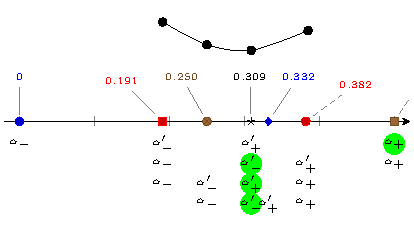
\includegraphics[width=0.85\textwidth]{tikzpics/zero_order.pdf}
		\caption{Plot of iterates of zero order algorithm for line search. The lines below the $x$ axis represent the different values of $\alpha_-, \alpha_+, \alpha'_-, \alpha'_+$ across different iterations, while the greed dot marks how the value $\alpha$ changes.}\label{fig:25ott_zero_order}
	\end{figure}

	Let us try \Cref{alg:25ottnonDeriv} on a toy example, displayed in \Cref{fig:25ott_zero_order}.
	Let $\alpha = 0$ and let $\eps = 1$.
	
	\[
	\begin{split}
		&\alpha_- = 0\\
		&\alpha_+ = 0.5\\
		&\alpha'_- = r \alpha  = (1 - 0.618) \cdot 0.5 = 0.191\\
		&\alpha'_+ = r \cdot \alpha = 0.618 \cdot 0.5 = 0.309\\
	\end{split}
	\]
	Since $0.5 - 0 < 1$ we enter the loop.
	According to the values of function $\varphi$ in $\alpha_-$ and $\alpha_+$ we enter the \emph{if} branch:
	\[
	\begin{split}
	&\alpha_- = \alpha'_- = 0.191\\
	&\alpha'_- = \alpha'_+ = 0.309\\
	&\alpha = \alpha'_+ = 0.309\\
	&\alpha'_+ = \alpha_- + r \cdot (\alpha_+ - \alpha_-) = 0.191 + 0.618 \cdot (0.5 - 0.191) = 0.382\\
	\end{split}
	\]
	Provided that $0.5 - 0.191 < 1$ we enter the loop.
	According to the values of function $\varphi$ in $\alpha_-$ and $\alpha_+$ we enter the \emph{else} branch:
	\[
	\begin{split}
	&\alpha_+ = \alpha'_+ = 0.382\\
	&\alpha'_+ = \alpha'_- = 0.309\\
	&\alpha = \alpha'_- = 0.309\\
	&\alpha'_- = \alpha_- + (1-r) \cdot (\alpha_+ - \alpha_-) = 0.191 + 0.309 \cdot (0.382 - 0.191) = 0.25\\
	\end{split}
	\]
	Provided that $0.382 - 0.191 < 1$ we enter the loop.
	According to the values of function $\varphi$ in $\alpha_-$ and $\alpha_+$ we enter the \emph{if} branch:
	\[
	\begin{split}
	&\alpha_- = \alpha'_- = 0.25\\
	&\alpha'_- = \alpha'_+ = 0.309\\
	&\alpha = \alpha'_+ = 0.309\\
	&\alpha'_+ = \alpha_- + r \cdot (\alpha_+ - \alpha_-) = 0.25 + 0.618 \cdot (0.382 - 0.25) = 0.332\\
	\end{split}
	\]
\end{example}

\subsubsection{Inexact line search}

In the rest of this lecture we will present a line search method to determine the maximum amount to move along a given search direction, starting with a relatively large estimate of the step size for movement along the search direction, and iteratively shrinking the step size (``backtracking'') until a decrease of the objective function is observed that adequately corresponds to the decrease that is expected, based on the local gradient of the objective function.

%\addpic{0.5}{pics/25ott/armijo01.pdf}{The dotted line represents the line which has as slope the derivative of $f$ in $\vect{x}$.}{fig:25ott3}

\begin{definition}[Armijo's condition]
  Let $\varphi:\R^+ \cup \{0\} \to \R$ such that $\varphi(\alpha) = f(\vect{x} + \alpha \vect{d})$.
  The \textbf{Armijo's condition} selects those real values $\alpha$ such that the function value in those points ($\varphi(\alpha)$)is smaller than the value of a line which passes through $0$ and is less steep than the tangent to the curve in such point.
  
  Formally, $\alpha \in \R$ satisfies \textbf{Armijo's condition} if for come \emph{control parameter} $0 < m_1 < (\ll) 1$ the following holds
  
  \[
    \varphi(\alpha)\leq y_a(\alpha) =\varphi(0) + m_1 \alpha \varphi'(0) ~ (A)
  \]
\end{definition}

\begin{figure}[h]
	\centering
	\subfigure[Armijo's condition leads to a line which is less steep than the tangent in $\alpha=0$.]{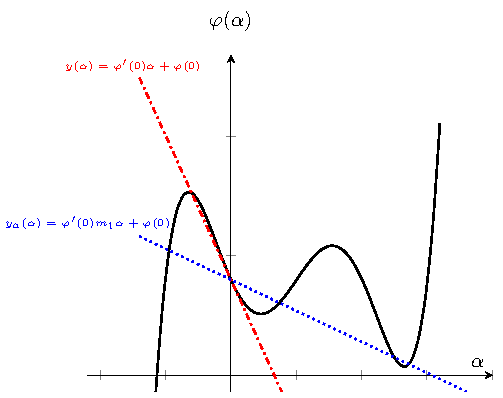
\includegraphics[width=0.45\textwidth]{tikzpics/armijo_2.pdf}\label{subfloat:armijo_2}}
	\hspace{0.5cm}
	\subfigure[Armijo's condition selects those $\alpha \in \R$ such that $\varphi(\alpha) < y_a(\alpha)$.]{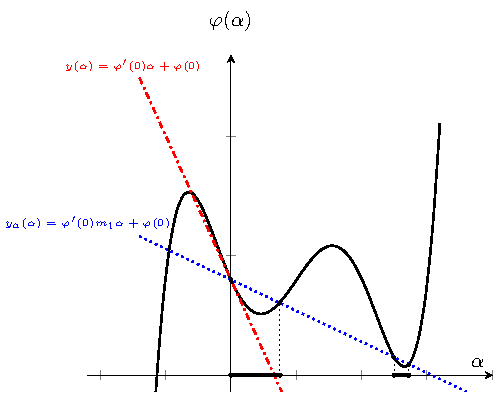
\includegraphics[width=0.45\textwidth]{tikzpics/armijo_3.pdf}\label{subfloat:armijo_3}}\\
	\caption{Graphical hint of the functioning of Armijo's condition.}\label{fig:armijo}
\end{figure}

Intuitively, provided that we are minimizing $\varphi$, $\varphi'(0) <0$.
This means that the slope of the line $y_a$ ($m_1 \varphi'(0)$) is smaller in absolute value (hence bigger) than the slope of the tangent to the curve $\varphi$ in $0$, therefore the line $y_a$ is less steep then $y$.

An attentive reader may notice that $\alpha \approx 0$ lead to values of $\varphi(\alpha) < y(\alpha)$, hence smaller than $y_a(\alpha)$, but this would lead to a very slow convergence.

\noindent In order to overcome this issue one can decide to start from a large $\alpha$ and reduce it until it satisfies Armijo's condition (as shown in \Cref{alg:25ottback}) or introduce another algebraic constraint:

\algo{alg:25ottback}{Pseudocode for backtracking line search.}{
	\Procedure{\bf BLS}{$\varphi, \varphi', \alpha, m_{1}, \tau$}
	\While{($\varphi(\alpha) > \varphi(0) + m_1 \alpha \varphi'(0)$)}
	\State{$\alpha \gets \tau \alpha$;}\Comment{With $\tau < 1$}
	\EndWhile%
	\EndProcedure%
}

%\addtwopics{0.4}{pics/25ott/armijo02.pdf}{0.4}{pics/25ott/armijo04.pdf}{In the left picture Armijo condition chooses a new line which slope is still negative, but less steep than the original one. In the right one, the ranges where to search are highlighted.}{fig:25ott4}

\begin{definition}[Goldstein's condition]
	Let $\varphi:\R^+ \cup \{0\} \to \R$ such that $\varphi(\alpha) = f(\vect{x} + \alpha \vect{d})$ and let $m_1 \in \R$ be the Armijo's constant.
	The \textbf{Goldstein's condition} selects those real values $\alpha$ that satisfy Armijo's condition but also such that the function value in those points ($\varphi(\alpha)$)is \emph{bigger} than the value of a line which passes through $0$ and is less steep than the tangent to the curve in such point.
	
	Formally, $\alpha \in \R$ satisfies the \textbf{Goldstein's condition} if for come \emph{control parameter} $m_1 < m_2 < 1$ the following holds
	
	\[
	\varphi(\alpha) \geq y_g(\alpha) = \varphi(0) + m_2 \alpha \varphi'(0) ~ (G)
	\]
\end{definition}

\begin{figure}[h]
	\centering
	\subfigure[Goldstein's condition leads to a line which is less steep than the tangent in $\alpha=0$ but steeper than Armijo's line.]{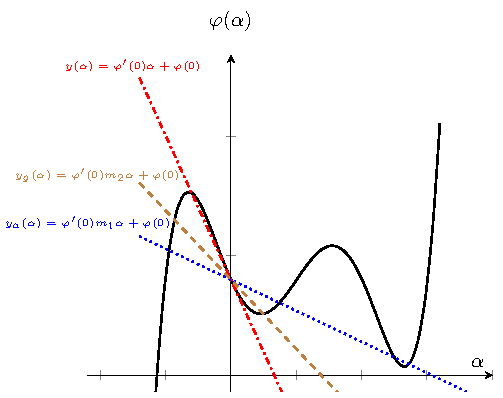
\includegraphics[width=0.45\textwidth]{tikzpics/goldstein_1.pdf}\label{subfloat:goldstein_1}}
	\hspace{0.5cm}
	\subfigure[Armijo's and Goldstein's conditions select those $\alpha \in \R$ such that $\varphi(\alpha) < y_a(\alpha)$ and  $\varphi(\alpha) > y_g(\alpha)$.]{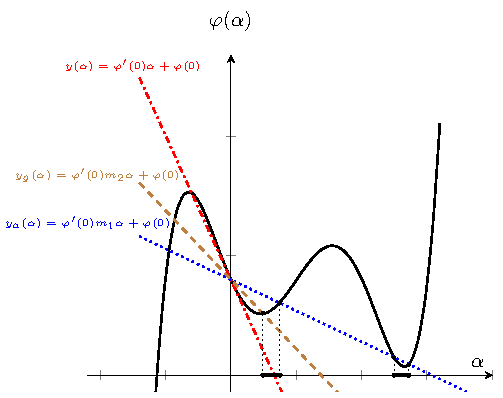
\includegraphics[width=0.45\textwidth]{tikzpics/goldstein_2.pdf}\label{subfloat:goldstein_2}}\\
	\caption{Conjunction of Armijo's and Goldstein's conditions.}\label{fig:goldstein}
\end{figure}

%\addpic{0.5}{pics/25ott/armijo05.pdf}{Goldstein condition chooses a new line which slope is still negative, less steep than the original one, but steeper than the one obtained by Armijo.}{fig:25ott5}

\noindent It may happen that the points that satisfy both Goldstein's and Armijo's conditions does not contain a local minimum.

%\addpic{0.5}{pics/25ott/armijo06.pdf}{Here are the intervals that satisfy both Armijo and Goldstein conditions.}{fig:25ott6}

\noindent To circumvent this problem another condition comes to help us.

\begin{definition}[Wolfe's condition]
	Let $\varphi:\R^+ \cup \{0\} \to \R$ such that $\varphi(\alpha) = f(\vect{x} + \alpha \vect{d})$ and let $m_1 \in \R$ be the Armijo's constant.
	The \textbf{Wolfe's condition} selects those real values $\alpha$ that allow for a decrease in the slope (\emph{curvature condition}), following the reasoning that close to the optimum the tangent line is almost horizontal.
	
	Formally, let $m_1 < m_3 < 1$
	\[
		\varphi'(\alpha) \geq m_3 \varphi'(0) ~ (W)
	\]
\end{definition}

\begin{figure}[h]
	\centering
	\subfigure[Wolfe's condition fixes a threshold for the slope of the line tangent to the curve $\varphi$.]{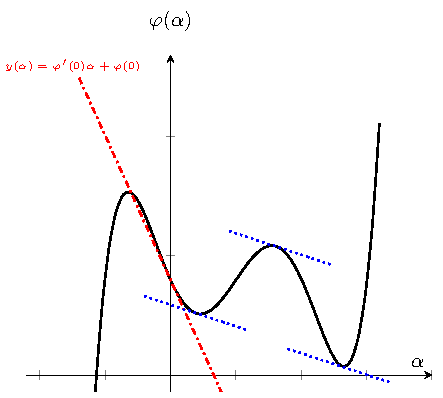
\includegraphics[width=0.45\textwidth]{tikzpics/wolfe_1.pdf}\label{subfloat:wolfe_1}}
	\hspace{0.5cm}
	\subfigure[Wolfe's rule selects those points where $\varphi'(\alpha)>0^-$.]{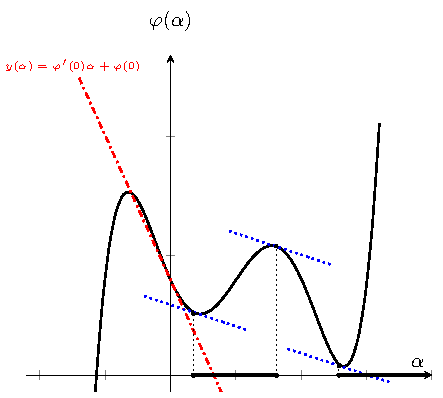
\includegraphics[width=0.45\textwidth]{tikzpics/wolfe_2.pdf}\label{subfloat:wolfe_2}}\\
	\caption{Wolfe's condition.}\label{fig:wolfe}
\end{figure}

\noindent \Cref{subfloat:wolfe_2} shows the intervals selected by Wolfe's rule.
Provided that we are moving along a direction of negative curvature for $f$, we have that $\varphi'(\alpha) < 0$, therefore Wolfe's condition is satisfied also by those points $\alpha$ where the derivative is positive.

Sometimes, the curvature condition is modified to force the step length to stay
in at least a broad neighborhood of a local minimizer or stationary point of the univariate function $\varphi$.

Provided that $\varphi'(0) < 0$, $\abs{\varphi'(0)} = -\varphi'(0)$; follows a stronger variant of Wolfe's condition.

%\addtwopics{0.4}{pics/25ott/armijo07.pdf}{0.4}{pics/25ott/armijo08.pdf}{On the left Wolfe condition (which chooses derivatives that are substantially zero). On the right part the intervals selected by Wolfe.}{fig:25ott7}

\begin{definition}[Strong Wolfe's condition]
	Let $\varphi:\R^+ \cup \{0\} \to \R$ such that $\varphi(\alpha) = f(\vect{x} + \alpha \vect{d})$ and let $m_1 \in \R$ be the Armijo's constant.
	The \textbf{strong Wolfe's condition} selects those real values $\alpha$ that allow for a decrease in the slope but prevent it to become big in absolute value.
	Formally, let $m_1 < m_3 < 1$
	
	\[
		\abs{\varphi'(\alpha)} \leq m_3 \abs{\varphi'(0)} = -m_3 \varphi'(0) ~ (W')
	\]
\end{definition}

\addpic{0.5}{tikzpics/wolfe_3.pdf}{Strong Wolfe's condition.}{fig:25ott8}

\begin{proposition}\label{prop:25ott}
	Let $\varphi:\R^+ \cup \{0\} \to \R$ such that $\varphi(\alpha) = f(\vect{x} + \alpha \vect{d})$.
	If $\varphi'(\alpha) \not\gg 0$ and both Armijo's and Wolfe's (or Armijo's and strong Wolfe's) conditions hold then all local minima (maxima) are captured unless $m_1$ is too close to $1$.
\end{proposition}

For a graphical hint of \Cref{prop:25ott}, see \Cref{fig:25ott9}, where we can observe that if $m_1 \approx 1$, the line is pretty steep, therefore the intersection between Armijo's and Wolfe's regions is very small.
In practice it is common to choose $m_1 \approx 0.0001$.

\addpic{0.5}{tikzpics/wolfe_4.pdf}{$m_1 \approx 1$ and the intersection between Armijo's and Wolfe's ranges.}{fig:25ott9}

The $m_{i}$ are like the hyperparameters of machine learning. Less formally, if we choose an $m_{1}$ far enough from $1$ everything works fine.

\begin{theorem}
Let $\varphi \in \C{1}$ and $\varphi(\alpha)$ bounded below for $\alpha \geq 0$ then $\exists ~ \alpha$ s.t.~(A) $\cap$ (W') holds.
\end{theorem}

\begin{proof}
	Let us write Armijo's line: $y_a(\alpha) = \varphi(0) + m_1 \varphi'(0)\alpha$.
	Let us define $d(\alpha) = y_a(\alpha) - \varphi(\alpha) =\varphi(0) + m_1 \varphi'(0)\alpha -\varphi(\alpha)$, such that $d'(\alpha) = y_a'(\alpha) - \varphi'(\alpha) = m_1 \varphi'(\alpha) - \varphi'(\alpha)= (m_1 -1) \varphi'(\alpha)$.
	It goes without saying that $d(0) = 0$ and $d'(0) = \underbrace{(m_1 - 1)}_{<1} \underbrace{\varphi'(0)}_{<1} > 0$.
	
	In $\alpha = 0$ the derivative of $\varphi$ is negative, hence the function $\varphi$ is decreasing.
	From the hypothesis we know that $\varphi$ is bounded below, hence at a certain point it will start increasing its value until it will intersect with Armijo's line eventually.
	Let us call $\bar{\alpha} > 0$ the smallest value such that $d(\bar{\alpha}) = 0$. All the points $\alpha \in ]0, \bar{\alpha}[$ satisfy Armijo's condition.
	
	\noindent We are left with the task of proving that also strong Wolfe's condition holds for those $\alpha \in ]0, \bar{\alpha}[$.
	$0$ and $\bar{\alpha}$ are the two roots of the function $d$, so we can use Rolle's theorem, in order to prove that the function $d$ has a stationary point in the interval $]0, \bar{\alpha}[$.
	Let us call the stationary point $\alpha^* \in ]0, \bar{\alpha}[$, $d'(\alpha^*)=0$ iif $\varphi'(\alpha^*) = - m_1 \varphi'(0)$, therefore $\abs{\varphi'(\alpha^*)} = m_1 \cdot \abs{\varphi'(0)}$ and this proves Wolfe's rule, because $m_1 < m_3 <1$, hence $\abs{\varphi'(\alpha^*)} \le m_3 \abs{\varphi'(0)}$.
\end{proof}

\addpic{0.5}{pics/25ott/3.png}{If $\varphi$ is not going to $-\infty$ the Armijo's line (blue) and the function will meet in $\bar{\alpha} > 0$.}{fig:25ott10}

How can we find such a point? 

\begin{proposition}\label{prop:lipshitz}
	Let $\varphi:\R^+ \cup \{0\} \to \R$ such that $\varphi(\alpha) = f(\vect{x} + \alpha \vect{d})$ and let $\nabla f$ be $L$-Lipschitz.
	Then $\varphi'$ is $L$-Lipschitz as well and $L$ does not depend on $x^i$.
\end{proposition}

\begin{proof}
	\[
	\begin{split}
		\abs{\varphi'(\alpha_1) - \varphi'(\alpha_2)} &= \abs{\tr{\vect{d}} \nabla f(\vect{x} +\alpha_1 \vect{d}) - \tr{\vect{d}} \nabla f(\vect{x} +\alpha_2 \vect{d})}\\
		&= \tr{\vect{d}} \underbrace{\abs{\nabla f(\vect{x} +\alpha_1 \vect{d}) - \nabla f(\vect{x} +\alpha_2 \vect{d})}}_{\le L \cdot \abs{\vect{x} + \alpha_1 \vect{d} - (\vect{x} +\alpha_2 \vect{d})}}\\
		&\le \tr{\vect{d}} L \cdot \abs{\cancel{\vect{x}} + \alpha_1 \vect{d} - (\cancel{\vect{x}} +\alpha_2 \vect{d})}\\
		&= \tr{\vect{d}} L \abs{\alpha_1 -\alpha_2} \vect{d}\\
		&\stareq L \cdot \abs{\alpha_1 - \alpha_2}
	\end{split}
	\]
	where $\stareq$ follows from the fact that $\vect{d}$ has norm $1$.
\end{proof}

\begin{proposition}
	Let $\varphi:\R^+ \cup \{0\} \to \R$ such that $\varphi(\alpha) = f(\vect{x} + \alpha \vect{d})$,  $\varphi$ bounded below and $\nabla f$ $L$-Lipschitz.
	$\bar{\alpha} \in \R$ has the same behaviour of $\norm{\nabla f(\vect{x^i})}$.
	Formally,
	\[
		\bar{\alpha} > (1 - m_1) \frac{\norm{\nabla f(\vect{x^i})}}{L}
	\]
\end{proposition}

\begin{proof}
	According to \Cref{prop:lipshitz}, $\varphi'$ is $L$-Lipschitz and
	\[
		L(\bar{\alpha} - 0) \geq \varphi'(\bar{\alpha}) - \varphi'(0) > (1 - m_1) (- \varphi'(0)) \stareq (1 - m_1) (\norm{\nabla f(\vect{x^i})}) 
	\]
	where $\stareq$ follows from 

	\[
	\varphi'(\alpha) = \ps{\nabla f(\vect{x} + \alpha \vect{d})}{\overbracket[0.5pt]{\eqmathbox{\mathstrut \vect{d}}}^{
			\eqmakebox[M][l]{\rlap{\footnotesize \hspace{-2cm}$ -\nabla f(\vect{x} + \alpha \vect{d})  / \norm{\nabla f(\vect{x} + \alpha \vect{d})}$}}}} = \frac{\sqrnorm{\nabla f(\vect{x} + \alpha \vect{d})}}{\norm{\nabla f(\vect{x} + \alpha \vect{d})}}
	\]
	therefore $	\bar{\alpha} > (1 - m_1) \frac{\norm{\nabla f(\vect{x^i})}}{L}$.
\end{proof}

Now we can prove the following

\begin{theorem}
  If (A) $\cap$ (W) holds $\forall i$ then either $\{f(\vect{x^i})\} \to -\infty$ or $ \{\norm{\nabla f(\vect{x^i})}\} \to 0$. 
\end{theorem}

\begin{proof}
  \textbf{By contraddiction}, we assume that $\norm{\nabla f(\vect{x^i})}$ diverges.
   Formally, $- \varphi'(0) = \norm{\nabla f(\vect{x^i})} \geq \varepsilon > 0 ~ \forall i$. Then
  \begin{enumerate}
    \item (W) $\Longrightarrow \alpha^i \geq \bar{\alpha} > (1 - m_1) \frac{\norm{\nabla f(\vect{x^i})}}{L}$. Let $\delta := \frac{(1-m_1) \cdot \eps}{L}$, then $\alpha^i \geq \delta > 0$;
    \item (A) $\Longrightarrow f(\vect{x^{i+1}}) \leq f(\vect{x^i}) - m_1 \alpha^i \norm{\nabla f(\vect{x^i})} \leq f(\vect{x^i}) - m_1 \delta \varepsilon$;
    \item So $\{f(\vect{x^i})\} \to -\infty$ (or $ \{\norm{\nabla f(\vect{x^i})}\} \to 0$).
  \end{enumerate}
\end{proof}

Backtracking is similar: for simplicity, $\alpha = 1$ (input)

      $\norm{\nabla f(\vect{x^i})} > \varepsilon \forall i \Longrightarrow \bar{\alpha} > \delta > 0 \forall i$

      $h = \min \{k : \tau^{-k} \leq \delta\} \Longrightarrow \alpha^i \geq \tau^{-h} > 0 \forall i \Longrightarrow$ $f(\vect{x^{i+1}}) \leq f(\vect{x^i}) - m_1 \tau^{-h} \varepsilon \Longrightarrow \{f(\vect{x^i})\} \to -\infty$ or \faFlash.
